\section{Discussion}

% @AML:
% - From GP results: hash metric most susceptible to mutational meltdowns

% \begin{figure}
\begin{center}

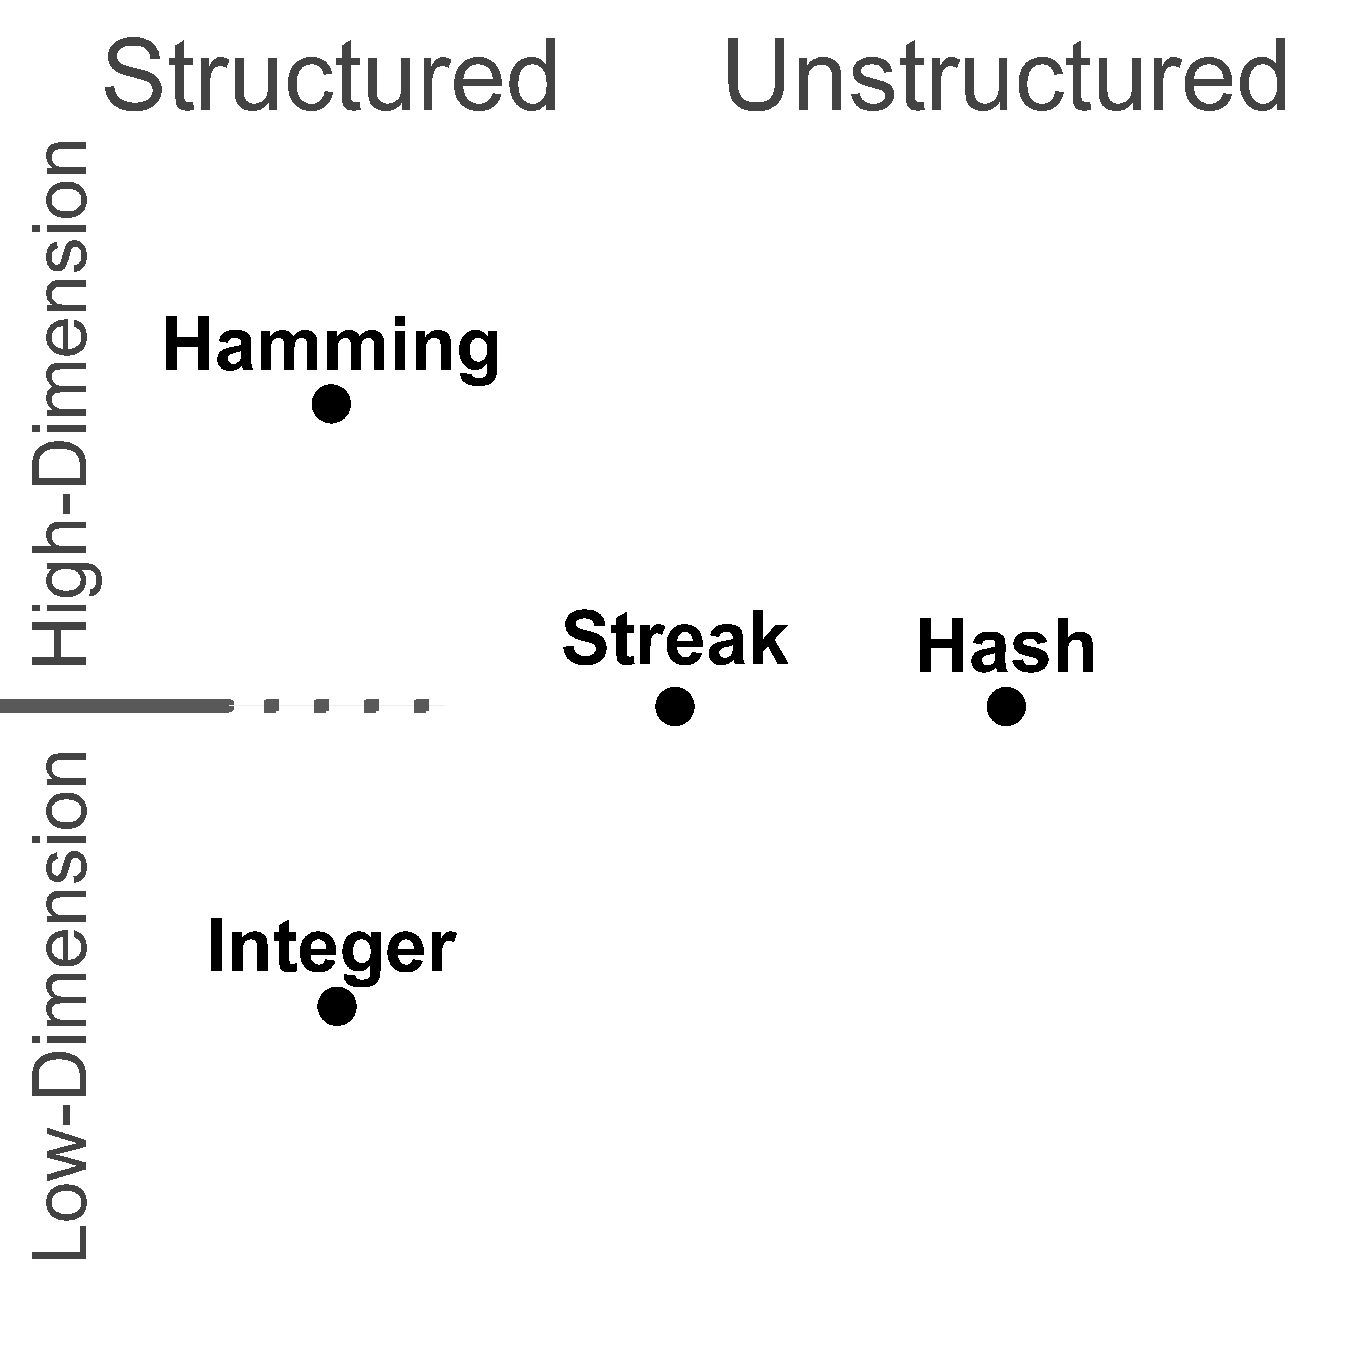
\includegraphics[width=\columnwidth]{{{img/conceptual-geometry}}}
\caption{
A conceptual schematic of the tag-matching metrics' geometric properties.
}
\label{fig:conceptual_geometry}

\end{center}
\end{figure}

% First, we performed  %TODO
% If two tags both closely match a third tag, will these two tags be constrained to closely match each other?
% Likewise, if a tag closely matches a second tag, will the tag be constrained to poorly match other tags the second tag poorly matches?
We used geometrical analyses to explore how tag-matching metrics constrain patterns of connectivity between tags, making some configurations unlikely or even impossible.
The bidirectional integer metric exhibited the tightest geometrical constraint in our analyses.
The unidirectional integer metric also exhibited tight geometrical constraint, but quirks of its non-commutative construction can allow that constraint to split across perfect- and worst-matching extremes.
Hamming and streak metrics exhibited looser geometric constraint, with the streak metric allowing for edge cases that very strongly break constraints.
Finally, the hash metric exhibited no geometrical constraint.

Next, we analyzed the effect of bitwise mutation on match distance score under the different metrics.
Under the hamming metric, all mutations have small effects on match distance score.
In contrast, under the integer metrics, rare mutations can have strong effects on match distance score.
The streak metric also exhibited strong-effect mutations, particularly with respect to coupling loosely-affiliated tags.
The hash metric exhibited the fattest tails of mutational magnitude, with strong-effect mutations occurring frequently.
Interestingly, the hash metric also exhibited sign-outcome frequencies that differed from the other metrics: mutations that decoupled tightly-matching tags and mutations that coupled loosely-matching tags were more frequent compared to other metrics.

The hamming metric exhibited the greatest robustness to mutation along mutational walks, followed by the streak metric.
The integer metrics, in particular the unidirectional integer metric, exhibited less robustness.
The streak metric, where all one-step mutations scramble match distance, exhibited the least robustness.

In evolutionary experiments, we found that network constraint (the number of tags a query or operand needs to simultaneously establish affinity with) influenced the relative performance of tag-matching metrics. 
% In target-matching evolutionary experiments, network constraint corresponded to degree and regularity of the target graphs.
% In the genetic programming experiments, network constraint corresponded to the interconnectedness of module interaction networks that were selected for.

In target-matching evolutionary experiments, we found that the hash metric enabled rapid adaptive evolution toward targets with low network constraint.
This rapid evolution may be due to the hash metric's ability to rapidly generate variation.
Under high network constraint, however, the hash metric yielded poor-quality solutions.
The integer metrics also yielded poor-quality solutions for target graphs with network constraint.
In some more-constrained cases, the streak metric enabled more rapid adaptive evolution than the hamming metric.
 

In genetic programming evolutionary experiments, we found that the hamming and streak metrics yielded successful solutions the most frequently.
On the directional signal task, which tends to require denser interaction networks, we found evidence that the streak metric enabled more rapid adaptive evolution than the hamming metric.

The hash metric had the next best performance in SignalGP experiments, yielding more solutions than the integer metrics, which performed comparably.
Although the hash metric performed best in low-constraint target-matching experiments, it was outperformed in low-constraint SignalGP experiments. 
This may be due to the presence of duplication and differentiation processes across SignalGP lineages, where instruction and module count can grow over time. 

\begin{figure}
\begin{center}

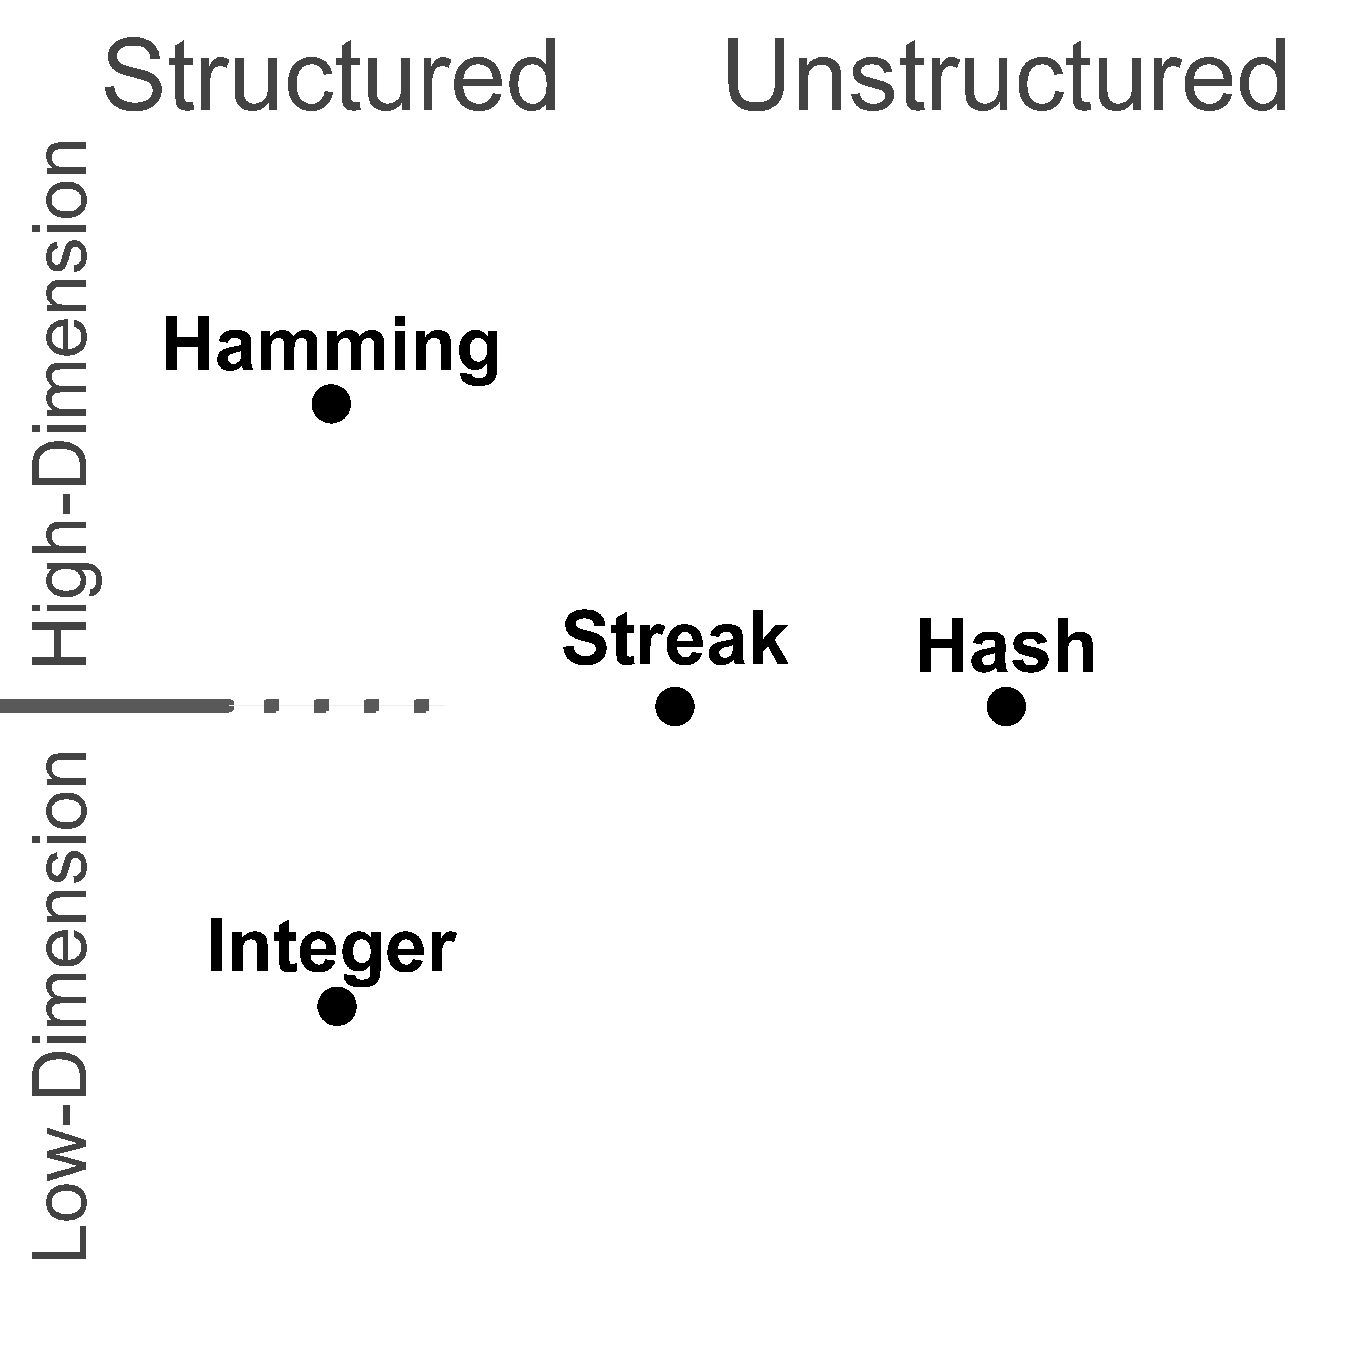
\includegraphics[width=\columnwidth]{{{img/conceptual-geometry}}}
\caption{
A conceptual schematic of the tag-matching metrics' geometric properties.
}
\label{fig:conceptual_geometry}

\end{center}
\end{figure}


Relative to the other metrics, the streak metric tends to offer intermediate variational and geometric properties.
Figure \ref{fig:conceptual_geometry} depicts a schematic summary of this observation.
It exhibits some, but not strict, geometric constraint.
Many mutations are neutral or near-neutral (like the integer and hamming metrics) but a fat tail of extreme-effect mutations also occur (like the hash metric).
The streak metric exhibits robustness under mutational walks that falls between the hamming and integer metrics.
These mechanistic observations offer a potential explanation for the streak metric's strong performance facilitating adaptive evolution under high-constraint conditions.
However, whether these mechanistic explanations are sufficiently complete --- especially with respect to the streak metric's outperformance of the hamming metric under high-constraint conditions --- is unclear.


